\subsection{Path Following with PID Controller}

It is better to complete this section in a flat panel display. As this part is more algorithm centered. Instead of using the DroneXrEmulator in \cref{fig:quad_structure}, it is simpler to make another PidDroneEmulator which maps the calculated joystick value to YueInputModule.

To implement path following, two other components are included, PathFollower, cut the path into different targets for PidDroneEmulator to calculate errors and PathGenerator to build the path.

To move between points, the PathGenerator generates a path using two Cubic Bézier curves. Given four control points $P_0, P_1, P_2, P_3$, home to waypoint and back, the position $B(t)$ for $t \in [0,1]$ is defined as \cref{eq:bezier}.

\begin{equation}\label{eq:bezier}
    B(t) = {(1-t)}^3 P_0 + 3{(1-t)}^2 t P_1 + 3(1-t) t^2 P_2 + t^3 P_3
\end{equation}

The path is constructed relative to the Home and Target vectors, the drone will fly from Home and fly back, the path as shown in \cref{fig:path_design}. Path from Home to Waypoint using a right-hand offset for control points; Path from Waypoint back to Home using a left-hand offset.

\begin{figure}[H]
    \caption{Path Design}\label{fig:path_design}
    \centering
    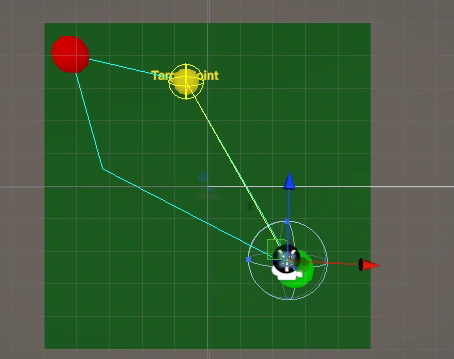
\includegraphics[width=0.8\linewidth]{img/path.png}
\end{figure}

By calculating these normalized joystick rates, the system can visualize the AI's calculation on the HUD.This serves as an AI collaboration hinter, showing human pilots the optimal stick positions for maintaining the designated path \cref{fig:pid-ui}.

\begin{figure}[H]
    \caption{hinter UI}\label{fig:pid-ui}
    \centering
    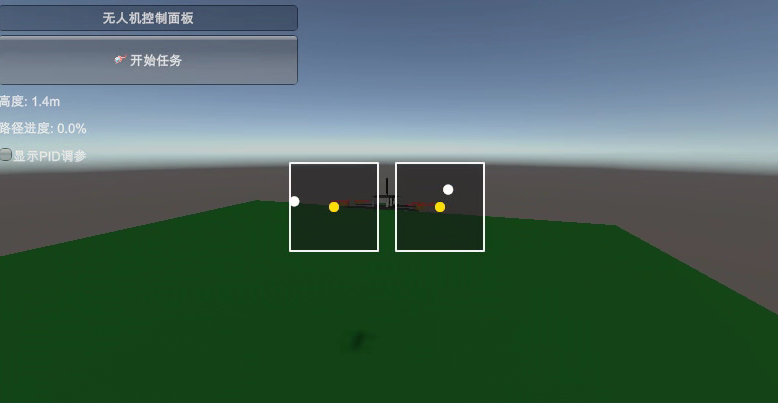
\includegraphics[width=0.8\linewidth]{img/ui.png}
\end{figure}

